%\documentclass{article}
\documentclass[12pt]{../SOP3}\usepackage[]{graphicx}\usepackage[]{color}
%% maxwidth is the original width if it is less than linewidth
%% otherwise use linewidth (to make sure the graphics do not exceed the margin)
\makeatletter
\def\maxwidth{ %
  \ifdim\Gin@nat@width>\linewidth
    \linewidth
  \else
    \Gin@nat@width
  \fi
}
\makeatother

\definecolor{fgcolor}{rgb}{0.345, 0.345, 0.345}
\newcommand{\hlnum}[1]{\textcolor[rgb]{0.686,0.059,0.569}{#1}}%
\newcommand{\hlstr}[1]{\textcolor[rgb]{0.192,0.494,0.8}{#1}}%
\newcommand{\hlcom}[1]{\textcolor[rgb]{0.678,0.584,0.686}{\textit{#1}}}%
\newcommand{\hlopt}[1]{\textcolor[rgb]{0,0,0}{#1}}%
\newcommand{\hlstd}[1]{\textcolor[rgb]{0.345,0.345,0.345}{#1}}%
\newcommand{\hlkwa}[1]{\textcolor[rgb]{0.161,0.373,0.58}{\textbf{#1}}}%
\newcommand{\hlkwb}[1]{\textcolor[rgb]{0.69,0.353,0.396}{#1}}%
\newcommand{\hlkwc}[1]{\textcolor[rgb]{0.333,0.667,0.333}{#1}}%
\newcommand{\hlkwd}[1]{\textcolor[rgb]{0.737,0.353,0.396}{\textbf{#1}}}%
\let\hlipl\hlkwb

\usepackage{framed}
\makeatletter
\newenvironment{kframe}{%
 \def\at@end@of@kframe{}%
 \ifinner\ifhmode%
  \def\at@end@of@kframe{\end{minipage}}%
  \begin{minipage}{\columnwidth}%
 \fi\fi%
 \def\FrameCommand##1{\hskip\@totalleftmargin \hskip-\fboxsep
 \colorbox{shadecolor}{##1}\hskip-\fboxsep
     % There is no \\@totalrightmargin, so:
     \hskip-\linewidth \hskip-\@totalleftmargin \hskip\columnwidth}%
 \MakeFramed {\advance\hsize-\width
   \@totalleftmargin\z@ \linewidth\hsize
   \@setminipage}}%
 {\par\unskip\endMakeFramed%
 \at@end@of@kframe}
\makeatother

\definecolor{shadecolor}{rgb}{.97, .97, .97}
\definecolor{messagecolor}{rgb}{0, 0, 0}
\definecolor{warningcolor}{rgb}{1, 0, 1}
\definecolor{errorcolor}{rgb}{1, 0, 0}
\newenvironment{knitrout}{}{} % an empty environment to be redefined in TeX

\usepackage{alltt}

%This area before it says begin is like the header area (preamble)


\author{Kristy Morris -- Revised: Virginia Paschal}
\title{SOP for In Vitro Determination of Chlorophyll \textit{a} Concentrations by Fluorescence}
\date{8/5/2016}
\approved{Los Huertos}
\ReviseDate{\today}
\SOPno{26 v.01}

\usepackage{graphicx}
\IfFileExists{upquote.sty}{\usepackage{upquote}}{}
\begin{document}


\maketitle

 \section{Scope and Application}

\NP This method provides a procedure for the fluorometric determination of chlorophyll \textit{a} and its magnesium-free derivative, pheophytin \textit{a} in marine and freshwater phytoplankton.

\NP This method is modified from the US EPA Method 445.0 and APHA Standard Methods for the Examination of Water and Wastewater, 22\textsuperscript{nd} Edition. 

\section{Summary of Method}

\NP Chlorophyll-containing phytoplankton in a measured volume of sample water are concentrated by filtering at low vacuum through a glass fiber filter (Whatman GF/F). The pigments are extracted from the phytoplankton in 90\% acetone and to ensure thorough extraction of chlorophyll \textit{a}, are allowed to steep for at least 2hrs. The fluorescence of the sample is measured at the excitation wavelength of 485 nm and emission wavelenghts 685 / 50 nm. Sample fluorescence is measured before and after acidification with 0.1 N HCl to obtain a corrected chlorophyll \textit{a} concentration. 


\section{Definitions}
\NP \textbf{Stock Standard Solution (SSS)} -- a solution prepared in the laboratory using reference materials purchased from a reputable commercial source.

\NP \textbf{Laboratory Reagent Blank (LRB)} -- an aliquot of reagent water (Milli-Q/SuperQ) or other blank matrices that are treated the same as the sample including exposure to all glassware, equipment, solvents, reagents, internal standards and surrogates that are used with other samples. The LRB is used to determine if method analytes or other interferences are present in the laboratory environment, reagents or apparatus. 

\NP \textbf{Field duplicates}-- Two separate samples collected at the same time and placed under identical circumstances and treated exactly the same throughout the field and laboratory procedures. Provide a measure of the precision associated with sample collection, preservation, storage and laboratory processing. 

\NP \textbf{Quality Control Samples (QCs)}-- A solution of known concentration obtained from a source external to the laboratory to check laboratory performance.

\NP \textbf{Linear Dynamic Range} -- The absolute quantity or concentration range over which the instrument response to the analyte is clear (basically, its the range of concentrations for which your fluorometer is suited to take accurate measurements). For the Turner Trilogy Fluorometer in Marc's lab the LDR is 0-1000 ppb RWT. 


\section{Interferences}
\NP Any substance extracted from the filter or acquired from laboratory contamination that fluoresces in the red region of the spectrum may interfere in the accurate measurement of both chlorophyll \textit{a} and pheophytin \textit{a}.

\NP Spectral interferences resulting from the fluorescence of the accessory pigment chlorophyll \textit{b}, and the chlorophyll \textit{a} degradation product pheophytin \textit{a}, can result in the overestimation of chlorophyll \textit{a} concentrations. However, highly selective optical filters used in this method minimize these interferences.

\NP Quenching effects are observed in highly concentrated solutions or in the presence of high concentrations of other chlorophylls and carotenoids. Samples should be diluted.

\NP Fluorescence is temperature dependent with higher sensitivity occurring at lower temperatures. Samples, standards, LRBS (section 3.2) and QCs (section 3.4) must be at the same temperature to prevent errors and maximize precision. Analysis of samples at ambient temperatures is required in this method.

\NP All photosynthetic pigments are light and temperature sensitive. Work must be performed in subdued light and all standards, QC materials and filter samples must be stored in the dark at -20\degree C to prevent degradation.

\section{Health and Safety}

\subsection*{Safety and Personnnel Protective Equipment}

\NP Lab safety-glasses and lab coats are required for all laboratory analysis. Use gloves to avoid skin irritation from contact with acetone; work under fume hood when possible. 

\NP Sonication Procedure -- When using the sonicator always wear ear protection. \textbf {Sonicator should never be used outside of solution.}

\NP Chemical Hygiene -- Please refer to the Safety Data Sheet files for questions concerning a chemical's toxicity and the necessary safety precautions.

\NP Waste Disposal-- Dispose of waste in the acetone collection bottle. See ''SOP 02 Handling of Hazardous Materials.'' %Figure out who and how this bottle will be disposed of properly. Most likely the Environmental Health and Safety Officer (Wang??) Ask Marc about what bottles he is planning to use to store organic and inorganic wastes.

\section{Personnel \& Training Responsibilities}

\NP Researcher training is required before the procedures in this method can be used... 

\NP Researchers using this SOP should be trained for the following SOPs:

\begin{itemize}
  \item SOP01 Laboratory Safety
  \item SOP02 Handing of Hazardous Materials
\item SOP 11 Preparing Standards and QCs %This is the one I think might be tricky because it's so generic. 
\end{itemize}

\section{Materials and Apparatus}

\NP Turner Designs Trilogy Fluorometer (P/N 998-7210)

\NP Whatmann glass micro fiber filter GF/F 0.7 $\mu$  m retention 47mm 

\NP Millipore glass filtration unit with vacuum and 47mm fritted glass disk base 

\NP Tweezers or flat tipped forceps

\NP Plastic petri dishes or some other solid container for storing sampled filters in the freezer

\NP Laboratory tissues (Kim wipes)

\NP Assorted class A calibrated pipettes 

\NP 50mL, 100mL, and 1-L class A volumetric flasks

\NP Sonicator or tissue grinders that have a teflon tipped pestle with grooves, a stainless steel rod (1/4" diameter) long enough to attach onto a suitable drive motor and a 30-mL capacity glass grinding tube

\NP Glass cuvettes for the fluorometer

\NP Desktop Clinical Centrifuge, capable of rotating 15mL tubes at 675 x g or 1,000 x g 

\NP 15 mL glass or polypropylene Falcon centrifuge tubes

\NP Aluminum foil

\NP Pastuer type pipettes or medicine droppers

\NP Polyethylene squirt bottles

\NP Room thermometer

\NP Note(for lab techs): All reusable labware that comes in contact with chlorophyll solutions should be cleaned with acetone and acid free. Dishwashing should include soaking in laboratory grade detergent and water, rinsing with tap water then rinsing with deionized water. 

\section{Reagents and Standards}
\NP Acetone, HPLC grade (CASRN 67-64-1)

\NP Concentrated Hydrochloric Acid (sp. gr. 1.19), (CASRN 7647-01-0)

\NP Chlorophyll \textit{a} free of chlorophyll \textit{b}. May be obtained from a commercial supplier.

\NP Milli-Q/Super-Q water

\NP \textbf{0.1 M HCl solution}-- Add 0.85 mL of concentrated HCl to approximately 50mL of water and dilute to 100 mL. 

\NP \textbf{Aqueous Acetone Solution}-- 90\% Acetone/ 10\% Milli-Q water. Carefully measure 100mL of water into a 100mL volumetric flask. Then pour the water into a 1L volumetric flask. Fill the 1L flask up to the line with acetone. Mix and then transfer to a dark amber bottle. Label the bottle and store in the flammables cabinet (under the middle fumehood in the Los Huertos Lab). 

\NP \textbf{Chlorophyll Standard Stock Solution (SSS)}- Chlorophyll \textit{a} from Sigma is shipped in an amber glass ampoule. This should be stored in the freezer until use. Tap the ampoule until all of the dried chlorophyll has settled on the bottom. Working in a darkened room, carefully break the tip off the ampoule and transfer the contents into a 50mL volumetric flask and dilute to volume with 90\% acetone (from section 8.6). Transfer to a darkened bottle or wrap the flask in foil to protect it from light. The concentration of the solution must be determined spectrophotometrically using a multiwavelength spectrophotometer. Label bottle including the chlorophyll lot number. When stored in an airtight container at room temperature, the SSS is stable for at least six months.

\NP \textbf{Chlorophyll \textit{a} Primary Dilution Standard (PDS)}- Add 1mL of the SSS (section 8.7) to a 100mL volumetric flask and dilute to volume with aqueous acetone solution (section 8.6). If exactly 1mg of pure chlorophyll was used to prepare the SSS, the concentration of the PDS is 200 $\mu$ g/L. Prepare fresh prior to use and label flask and wrap in foil.

\NP \textbf{Quality Control Samples (QCs)}- Since there are no commercially available QCs, they must be prepared from the PDS at the following concentrations:
\begin{itemize}
\item QC1 = 5 $\mu$ g/L
\item QC1 = 20 $\mu$ g/L
\item QC1 = 50$\mu$ g/L
\item QC1 = 200 $\mu$ g/L
\end{itemize}

\section{Estimated Time}

\NP This procedure requires XX minutes...

\section{Procedure} 

% Using \subsection to split extraction and analysis

\subsection*{Filtration}
\NP Invert the sample bottle gently several times before filtering to suspend particles. Mixing the sample well improves the replication greatly.


\NP\textbf{The below image demonstrates the correct setup of the filtration system.}

\begin{figure}[h!]
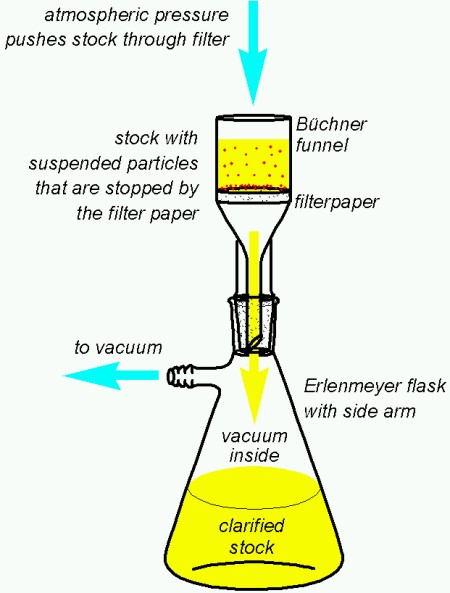
\includegraphics[width=.5\linewidth]{Filtersetup.jpg}
\end{figure}

The filtration system is comprised of four parts: the Erlenmeyer flask, the glass funnel, the bottomless beaker, and the aluminum spring clamp. 
\begin{itemize}
\item Slide the glass funnel on top of the Erlenmeyer flask.
\item Use tweezers to set a filter paper over the glass funnel.
\item Carefully set the bottomless beaker over the glass funnel making sure the filter remains centered in place. 
\item Use the aluminum spring clamp to secure the beaker to the funnel while still making sure the filter paper does not move. \item Attach the hose of the vacuum to the vacuum outlet of the glass filter.
\item Turn the vacuum on. 
\end{itemize}






\NP \textbf{Conduct filtration in an area with subdued light.} Gently filter the sample in 20 mL increments using a graduated cylinder or calibrated pipette. The volume to be filtered will vary depending on the algal concentration in the sample. The sample needs to be filtered just until a brown or green tint is visible on the filter. ({\small \textit{Note: For benthic samples a much smaller volume will need to be filtered, roughly 5mL. For freshwater samples the volume can range from 20mL to 300mL, and seawater sample volume can exceed 1 L.}})

\NP Record the filtered sample volume during this process. If the filter is too green the sample analysis will be over range and will need to be diluted later.  It is best to avoid diluting the sample when possible. 

\NP After filtration, use forceps and a micro spatula to fold each filter in half with the analyte portion inside. Gently blot excess water with on the outside of the filter with a kim wipe. Place the filter inside a clean 15mL falcon tube or plastic petri dish.  
\NP Remember to perform a laboratory duplicate and blank (100mL Milli-Q) every 10-15 samples.

\NP You can freeze the filter samples for up to 28 days before extraction. Be sure to wrap the petri dishes or falcon tubes with aluminum foil before storing to protect the chlorophyll from light. 

\subsection*{Extraction}

\NP Remove samples from the freezer and allow both the sample and QCs to come to room temperature

\NP There are two different methods used to extract chlorophyll from the glass fiber filters: the sonicator method and the tissue grinder method. If using a sonicator proceed on to the next section, if using a tissue grinder skip to section 10.10

\NP To extract chlorophyll \textit{a} via sonication method:
\\ \textbf{Ear plugs or ear muffs should be worn at all times when the sonicator is in use.}
\begin{itemize}
\item Add 25 mL of 90\% aqueous acetone solution to the falcon tubes ensuring each filter is fully submerged in the solvent. (The sonication procedure is usually done in 50 mL Falcon tubes)
\item Cap the tubes and invert several times to mix. 
\item Secure sonicator into clamp and stand. 
\item Turn on by pressing the | symbol. Turn off by pressing the O symbol.
\item Set sonicator to 70\% amplitude. 
\item  Sonicate by sumberging the tip of the sonicator halfway into the acetone solution. To help break up the filter completely, be sure to move tip around the entire sample.
\item After sonication, vigorously shake sample several times, cover with foil and then steep in a fridge (4\celsius) for at least 2 hrs.
\end{itemize}

\NP To extract a chlorophyll sample via tissue grinder method: 
\begin{itemize}
\item Using forceps remove the filter from its container and place it into the 30 mL glass grinding tube.
\item Push the filter to the bottom of tube using the pestle or a glass rod.
\item Using a volumetric pipette (with a tip suitable for dispensing acetone) add 4 mL of 90\% aqueous acetone solution to the tube.
\item Grind the sample using the pestle (and if applicable a tissue homogenizer motor) until it has been converted to a slurry. (Note: care must be taken not to overheat the sample in the process of grinding. Use common sense in deciding when the sample has been mascerated sufficiently.)
\item Pour the slurry into a 15 mL screw-cap centrifuge tube. 
\item Rinse the pestle and grinding tube with 6 mL 90\% aqueous acetone solution and add the slurry to the 15 mL centrifuge tube.
\item Cap the 15 ml centrifuge tube and shake it vigorously. After labeling and wrapping the tube in foil allow the sample to steep in the fridge (4/celsius) for 2 hours.
\item Before grinding a subsequent filter, clean out the grinding tube and pestle by rinsing with the water and acetone squirt bottles. The last rinse should be with acetone. Wipe the pestle from any leftover residue using a kim wipe.
\end{itemize}

\NP After the steeping period take the samples out from the fridge and allow them to come to room temperature. (This should take about 30 mins). A constant temperature water bath can be used.

\NP Shake the samples vigorously again and then using the clinical benchtop centrifuge centrifuge the samples at 1,000 x g for 5 minutes or until all filter material is separated from the extration liquid. Be sure to use the fixed angle buckets (45\degree) and the appropriate settings on the centrifuge to set the correct RCF. 

\NP When removing the tubes from the centrifuge, be careful not to re-suspend filter particles from the bottom of the tubes.

% the settings for the centrifuge will have to be configured based on the new equipment, need to calculate the correct g force but will need the centrifuges rotational radius for this. (the large one already calculates it). 

\subsection*{Sample Analysis}

\NP 2.5 mL of supernatant from each sample will be dispensed into a clean glass cuvette, again taking care not to resuspend filter particles.

\NP Turn on the fluorometer (back left side) and allow 10 minutes for warmup countdown to complete. 

\NP Turn on the lab computer and open SIS for Turner software to record data. 
\begin{itemize}
\item After launching the SIS for Turner program, you should get a pop up window. In that pop up window click the boxes next to COM 1 and MS Excel.
\item After pressing start the program should launch Microsoft Excel Automatically.
\item This program will make it easy to keep track of and save data for all your samples
\end{itemize}

\NP Next you will use the touchscreen on the Turner Fluorometer to select the correct module for analyzing your chlorophyll \textit{a} samples. Select the "Chlor-A" module from the choices on the screen. {\small \textit{Note: The ``Chlor-A" module stands for ``Chlorophyll Acidified". This is the correct setting for analyzing chlorophyll samples that will be acidified in order to obtain a corrected chlorophyll a concentration and a pheophytin a concentration. The module ``Chlor-NA" can be used to analyze chlorophyll samples that are NOT ACIDIFIED, however this will require that you repalce the snap in module inside the fluorometer to the appropriate one for analyzing non-acidified chlorophyll samples. The Chlor-NA module uses special band pass filters to automatically correct for interference from pheophytin a. The only drawback to using this alternative method is that you cannot get a pheophytin a concentration, only the concentration of chlorophyll a.}}

\NP Prior to measuring the fluorescence of your samples, you may need calibrate the fluorometer. A calibration will be performed using the the QCs made from the PDS (see definitions in Section 3). Read and record the values for the QCs prior to sample analysis, according to the directions for a Direct Multipoint Calibration found in the Turner Trilogy Fluorometer User's Manual pg. 20-22). If you're not performing your own calibration select a saved calibration from the menu in the "tools" setting.

\NP Use the 90\% acetone solution for a blank measurement.


\NP Wipe the outside of the cuvette with a kimwipe before taking a measurement then press measure the raw fluorescence of the sample. If the chlorophyll \textit{a} concentration of a sample is within 90\% of the upper limit of the LDR (which is 1,000 $\mu$ g/L for the Turner Trilogy fluorometer) it will be necessary to perform a dilution. However, samples should not be over diluted so be sure to use an appropriate dilution factor. 

\begin{description} 
\item[For a 1:2 Dilution] Simply add a 1 mL aliquot of the sample into 1 mL aqueous acetone solution.
\item[For a 1:100 Dilution] If the concentration of chlorophyll \textit{a} in the sample is very high you can try this dilution factor. Add 50 $\mu$ L of sample to 4.95 mL of aqueous acetone solution. 
\end{description}

\NP It will be necessary to calculate corrected chlorophyll \textit{a} values to determine whether dilutions need to be made. This is because pheophytin \textit{a} concentrations will not be the same across all samples. An excel spreadsheet template with equations can be found on %....some place in sakai or github that we haven't created yet

\NP After reading the fluoresence of all samples, add 75 $\mu$ L of  0.1M HCl to eah tube. Thoroughly mix the sample by sealing cuvette with a rubber stopper and inverting several times.Allow 90 seconds before measuring the fluorescence of all the samples again. 
% Don't thing we have a rubber stoper for the cuvettes can we use parafilm instead? 

\section{Data Analysis and Calculations}
To calculate 'corrected chlorophyll \textit{a}' values use the following equations: %fix the single opening quote

\NP Variables
\begin{enumerate}
\item $[Std]$ = Expected Standard concentration (This is not calculated, use the concentration of one of the standards that are run with the samples and it's corresponding F value)
%need to define what an F value is
\item $S_b$ = Standard reading before acidification
\item $S_a$ Standard reading after acidification
\item $F_b$ reading before acidification
\item $F_a$ reading after acidification
\item $V_e$ volume of extract
\item $V_s$ volume of sample 
\end{enumerate}

\NP Equations
\begin{description}
\item[Equation 1:] Acid Ratio (AR) = ($S_b$-Blank)/($S_a$-Blank)
\item[Equation 2:] Interpolation Before (InterpB) = $[Std]$*($F_b$-Blank)/($S_b$-Blank)
\item[Equation 3:] Interpolation After (InterpA) = $[Std]$*($F_a$-Blank)/($S_b$-Blank)
\item[Equation 4:] Corrected Chlorophyll \textit{a} = $[AR/(AR-1)]$*(InterpB-InterpA)*($V_e/V_s$)
\item[Equation 5:] Corrected Pheophytin \textit{a} = ((AR*InterpA)-InterpB)*($V_e/V_s$)
\end{description}
Note: Generally, equation 5 is not used. 

\section{QC/QA Criteria}

\NP An LRB is performed every 10 samples. The LRB should be less than the calculated lower detection limit for analysis.

\NP The QCs should be within $\pm$ 20\% of the known value. 

\NP The RSD of the replicate measurements should be within $\pm$ 20\%


\end{document}
